% Technical background}
\chapter{Technical background}
\label{Technical}

\lhead{Chapter 2. \emph{Technical background}}

\section{VLC Standard}
VLC as we know it today would not be possible without LEDs. Before we introduce
our proposal, we provide background information
about LEDs as wireless transmitter, then we describe the many ways in which
light intensity can be modulated and received, and the lice coding scheme used
in indoor VLC.



\section{VLC Technology}

Modulation of light has been used for centuries. In 1792 the French inventor
Claude Chappe invented the optical telegraph, a system of towers with signaling
devices, which allowed Napoleon to pass messages throughout his empire. Although
simple and practical, these systems are the ancestors of VLC. For some decades
after these events, light communication in the form of morse was used, but further
development of light communication stood still because with incandescent lamps
the data rates pale in comparison to what could be achieved with radio.

It is only until recently that we have a pervasive infrastructure that can modulate
light to achieve data rates that are meaningful for today’s communication needs.
Due to recent advancements in LED technology we can transform light bulbs into
high speed wireless transmitters. Data can be modulated in every light source
using changes in intensity, but only certain light sources possess the necessary
properties to transmit high data rates.

Fundamentally, modulating light requires changes of light intensity. For the last
century incandescent lamps have been the primary source of light, but incandescent
light cannot comply with high speed modulation because of the mechanism
it uses to generate light. Incandescence is the effect of emitting thermal radiation
from matter as a result of its temperature. In incandescent light bulbs a wire is
heated by running a current through it, and the resistance of this wire forms kinetic 
energy which is released in the form of light. This means that intensity control
of incandescent lamps takes place through two steps, resulting in indirect control
of the signal. This would not be a problem if the thermal inertia would not make
the system too slow for high speed modulation, but it does.

In the case of LEDs, the direct relation between intensity and electricity permit
high speed modulation. LEDs consist of a semiconductor material that contains
excited electrons. A fundamental property of electrons is that when they are
forced into a lower energy state they release their energy in the form of the emission
of photons. This effect is called electroluminescense and gives direct control
over light intensity through the control of voltage and current. A simple circuit
with transistors can deliver the necessary control of current, and this makes the
changes in light intensity fast enough to transfer information at a high data rate.

An alternative to LEDs is laser. Lasers can also be controlled at high speed, and
have the additional capability of strengthening the electroluminescense effect by
amplifying and focusing the generated light. This makes laser a good candidate
for long range communication, but for short distances its transmission angle is too
narrow (and hence it can be easily obstructed) without using lenses. Another
important disadvantage of laser is that poses health hazards to human beings.

\subsection{Modulation and transmitter}

The light emitted by LEDs can be modulated in different forms, and there are also
several types of receivers that can be used to decode the modulated light. Next,
we describe all these options.

As mentioned before, the ability of LEDs to modulate light at high speeds make
them the obvious choice for VLC transmitters in terms of speed and light intensity,
but potentially good transmitters are not the only thing that make a communication
system work. Data needs to be encoded (or modulated) into a signal before
transmission.
In radio communication, two common parameters used in signal modulation
are amplitude and frequency. Although radio and light are both electromagnetic
waves, the effect of modulation is not the same. We will briefly describe this point
to make the reader aware of the fundamental difference in modulation between
radio and VLC.

In radio, frequency modulation changes the frequency of the waves in the electromagnetic
field, and amplitude modulation changes the height of this waves.
In VLC, amplitude modulation works the same way as in radio, and it is often
called intensity modulation. Frequency modulation however, is very hard to apply
with visible light. It can be done but requires advanced laser setups to change
the signal’s properties, like phase and frequency, through interference. Instead,
when people talk about frequency modulation in VLC, they mean that the intensity
is shaped into a high frequency signal. By varying the frequency of this intensity
pulses, we get frequency modulation.

So, frequency modulation in VLC is actually frequency modulation through amplitude
modulation. This is the main difference between radio and light modulation.

There are many different modulation schemes in use for VLC, and we will now
discuss the most commonly used.

\begin{enumerate}

\item On-Off-Keying (OOK), or amplitude shift keying, uses keying (switching) to
turn a carrier signal on and off. OOK has a low processing burden but is
proven to be very sensitive to noise. Enhanced schemes like On-Off-Keying
Non-Return-to-Zero have shown data rates of 1.5 Gigabits per seconds,
using a Integrated Circuit with LEDs bonded into the chip \citep{ook-450}.

\item Pulse Time Modulation (PTM) is a technique in which data is modulated
in the ratio between the on and off time of the carrier signal. Pulse Position
Modulation (PPM) and Pulse Width Modulation (PWM) fall into this
category. The advantage of PTM is that it does not require digital-to-analog
converters to generate a smooth output signal, and does not require an
analog-to-digital converter either but only a comparator circuit. On the other
hand, PTM requires accurate timing for both the receiver and transmitter
because the ratio between on and off periods needs to be well synchronized.
Another advantage of PTM is that it provides flickering and dimming
support without additional techniques, which is good for use in illumination
devices, but speeds are lower than with other modulation systems \citep{ppm}.


\item  Pulse Amplitude Modulation (PAM) uses brightness levels to realize multilevel
signals to encode symbols. This modulation is sensitive to external
light sources as they influence the intensity, and has relative low speeds
compared to other techniques. Dimming control can easily be implemented
in PAM by changing the probability of the constellation points \citep{diming}
iv Frequency Shift Keying (FSK) looks a lot like On-Off-Keying, but instead of
switching a carrier on and off, the system switches between two frequencies.
This switch in frequency can be in terms of color i.e. a one is red and
a zero is blue, or in pulse frequency.

\item Phase Shift Keying (PSK) encodes symbols by changing the phase of the
light intensity that has been shaped into a sinusoidal form. Many variants
of PSK exist, depending on the number of constellation points used (Binary
PSK uses 2 points, 0\degree  and 180\degree , Quadrature PSK uses 4 points). PSK
can be used as base modulation, but can also be used in combination
with other techniques like OFDM to improve certain weaknesses like intersymbol
interference \citep{ofdm-plc}.

\item Orthogonal Frequency Division Multiplexing (OFDM) is a technique that
uses a large number of modulated carriers with sufficient frequency spacing
so that they are orthogonal. Again, this frequency is modulated through intensity.
The strongest advantage of OFDM is that it provides resistance to
multipath effects, which result in long distances and high speed data transfers.
Data rates beyond 3 Gigabit per seconds have been reported at short
distances $\approx$ 10cm) \citep{modulationStandard}. Unfortunately such high speeds demand require
high-speed processing units.

\item  Quadrature Amplitude Modulation (QAM) is a modulation scheme that conveys
bit streams by changing the amplitudes of two or more independent
carrier signals, which results in a spectral efficient scheme. A form of
QAM is the Carrier-less Amplitude and Phase (CAP) modulation, a promising
high speed VLC modulation scheme capable of transmitting at 3.22
gigabits per second using an RGB-type led. QAM and CAP can both
be combined with OFDM to improve its performance even further \citep{ofdm-cap}.

To select a good modulation scheme, people have designed models that can
be used to compare different schemes by simulating environmental conditions.
The Matlab-based platform of De Lausnay et al. evaluates different modulation
techniques and can also help to select the right modulation type \citep{matlab}.

Based on the information above, we decided to use On-Off-Keying modulation
for our platform because of the good average performance. The use of this technique keeps component count low so that multiple transmitters and receivers fit on the board.

\end{enumerate}

\subsection{Receivers}

While on the transmitter side the most widely used element is the LED, on the
receiver side we have several options: cameras, photodiodes and phototransistors,
and LEDs themselves. The common name for these types of sensors is
photodetectors and they use the same fundamental principle, the photoelectric
effect: many metals release electrons when light shines upon it. Although these
sensors share the same effect, they have subtle differences that result in unique
characteristics.

\begin{enumerate}

\item Cameras can detect light, its intensity and its color, using an array of semiconductor
junctions or capacitors. As the miniaturization of cameras continues
they can be found in embedded systems like mobile phones, allowing
them to receive vlc signals without additional hardware \cite{camera}. Cameras have
the advantage of focusing on the transmission source by looking at specific
pixels, so it becomes possible to select a specific VLC source or to ignore
a noise source. As a receiver for VLC, cameras have the disadvantage
of requiring more processing to retrieve the signal from the image sensor.
Secondly, a bigger disadvantage is the frame rate which is limited by the
camera’s (electronic or mechanic) shutter speed, which limits the signal
sample rate and thus the data transfer rate. There are high speed
cameras which offer a solution to this problem, but currently they are
too big and power hungry to use in embedded devices.

\item Photodiodes and phototransistors work based on the same principle but
their assembly is different: photodiodes have only one metal junction and
transistors have two. This semiconductor junction is exposed through a
transparent casing, so photons can reach the junction and, when having
the right frequency, excite electron-hole pairs which results in a current and
voltage. Because of the big surface of the semiconductor junction, photodiodes
and phototransistors are very sensitive to light. When comparing
photodiodes to phototransistors, diodes are faster due to the single junction
giving it a fast response time. On the other hand, phototransistors have a
bigger signal gain which results in a stronger electric signal. A disadvantage
of photodiodes is the dedicated circuitry needed for amplification, filtering
and sampling to be able to receive a clear electronic signal. Advances in
technology are capable of integrating these into a single chip which can
alleviate this disadvantage.

\item LEDs can be used as light sensors. An attentive reader may have noticed that photodiodes and LEDs exploit an oppose effect: while in photodiodes photons that strike the material generate a flow of electrons, in LEDs a flow of electrons release photons (light). This reversed and complementary effect can be used to make an LED both a receiver and a transmitter of VLC \citep{led2led}.

Considering the various options for receivers, we opted for photodiodes because
they have the higher potential to achieve high data rates, are more sensitive
than other sensors.

\end{enumerate}

\subsection{Line coding}

IEEE 802.15.7 standard suggests use different lines for VLC PHY I, that can be use with OOK or VVMN modulation.

\subsubsection{Manchester}

\subsubsection{4B6B}

\subsubsection{8B10B}


\section{Ara Plateform}
\subsection{Introduction to the Ara project}

Project Ara is the codename for an initiative that aims to develop an open hardware platform for creating highly modular smartphones. The platform will include a structural frame or endoskeleton that holds smartphone modules of the owner's choice, such as a display, camera or an extra battery. It would allow users to swap out malfunctioning modules or upgrade individual modules as innovations emerge, providing longer lifetime cycles for the handset, and potentially reducing electronic waste. Project Ara smartphone will begin pilot testing in Puerto Rico later 2015 with a target bill of materials cost of \$ 50 for a basic grey phone. The project was originally headed by the Advanced Technologies and Projects team within Motorola Mobility while it was a subsidiary of Google. Although Google had sold Motorola to Lenovo, it is retaining the project team who will work under the direction of the Android division.

\subsection{Project goals}
Google says the device is designed to be utilized by "6 billion people"; including 1 billion current smartphone users, 5 billion feature phone users, and 1 billion future user not currently connected. Google intends to sell a starter kit where the bill of materials is \$ 50 and includes a frame, display, battery, low-end CPU and WiFi.

Google wants Project Ara to lower the entry barrier for phone hardware manufacturers so there could be "hundreds of thousands of developers" instead of the current handful of big manufacturers. This would be similar to how the Google Play Store is structured. Lowering the barrier for entry allows many more people to develop modules. Anyone will be able to build a module without requiring a license or paying a fee.

\subsection{Structure and features}

Ara Smartphones are built using modules inserted into metal endoskeletal frames known as "endos". The frame will be the only component in an Ara Smartphone made by Google.It acts as the switch to the on-device network linking all the modules together. Two frame sizes will be available at first: "mini", a frame about the size of a Nokia 3310 and "medium", about the size of a LG Nexus 5.In the future, a "large" frame about the size of a Samsung Galaxy Note 3 will be available. Frames have slots on the front for the display and other modules. On the back are additional slots for modules. The data from the modules can be transferred at up to 10 gbps connection. The 2x2 modules have two connections and will allow up to 20 gbps. However, this stack isn't yet included in the Ara Development Kit, that only uses standard I/O such as UART or I2C, providing lower transfer rate.

Modules can provide common smartphone features, such as cameras and speakers, but can also provide more specialized features, such as medical devices, receipt printers, laser pointers, pico projectors, night vision sensors, or game controller buttons. Each slot on the frame will accept any module of the correct size. The front slots are of various heights and take up the whole width of the frame. The rear slots come in standard sizes of 1x1, 1x2 and 2x2. Modules can be hot-swapped without turning the phone off. The frame also includes a small backup battery so the main battery can be hot-swapped.Modules are secured with electropermanent magnets. The enclosures of the modules were planned to be 3D-printed, but due to the lack of development in the technology Google opted instead for a customizable molded case.

Modules will be available both at an official Google store and at third-party stores. Ara Smartphones will only accept official modules by default, but users can change a software setting to enable unofficial modules. This is similar to how Android handles app installations.

\subsection{Project team}

Project Ara was developed and is led by Paul Eremenko from Google ATAP. The core Project Ara team at Google consists of three people with most of the work being done by outside contractors. One of the main contractors is NK Labs, a Massachusetts-based engineering firm, whose co-founder is Ara Knaian after whom the project was named. Another contractor is 3D System.

\subsection{History and development process}

The first version of the developers' kit relies on a prototype implementation of the Ara on-device network using the MIPI UniPro protocol implemented on FPGA and running over an LVDS physical layer with modules connecting via retractable pins. Subsequent versions will soon be built around a much more efficient and higher performance ASIC implementation of UniPro, running over a capacitive M-PHY physical layer.
         
\subsection{Architecture}

\subsubsection{Android AP board}

The Application Processor Board is development kit for the Android Operating system giving convenient way to modify or update the OS.

The plateform is base

\begin{figure}[htbp]
  \centering
    \scalebox{0.4}{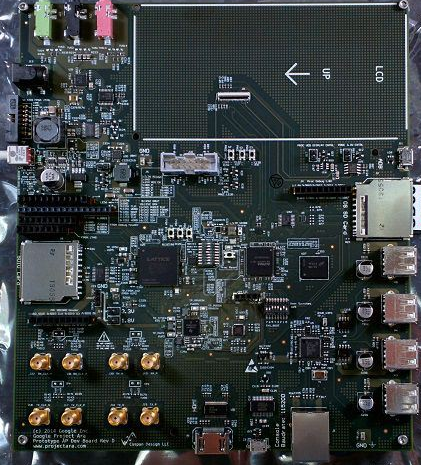
\includegraphics[width=\textwidth]{Pictures/APDevBoard.png}}
    \rule{35em}{0.5pt}
  \caption[Ara Application Processor Board]{Ara Application Processor Board}
  \label{fig:ap-board}
\end{figure}

\subsubsection{Endoskeleton}

\begin{figure}[htbp]
  \centering
    \scalebox{0.4}{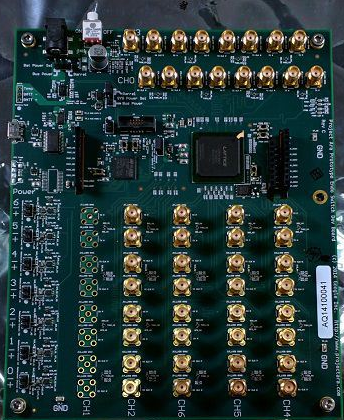
\includegraphics[width=\textwidth]{Pictures/endo.png}}
    \rule{35em}{0.5pt}
  \caption[Ara Endoskeleton Switch Board]{Ara Endoskeleton Switch Board}
  \label{fig:endo}
\end{figure}

\subsubsection{GP Endpoint board}

\begin{figure}[htbp]
  \centering
    \scalebox{0.4}{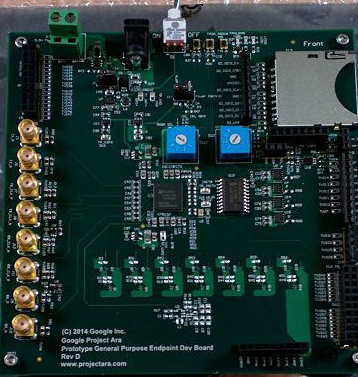
\includegraphics[width=\textwidth]{Pictures/genericendpoint.png}}
    \rule{35em}{0.5pt}
  \caption[Ara Generic Endpoint Board]{Ara Generic Endpoint Board}
  \label{fig:gpendpoint}
\end{figure}

